\documentclass[tikz,border=5pt]{standalone}
\usepackage[utf8]{inputenc}
\usepackage{tikz}
\usetikzlibrary{shapes.geometric, arrows.meta, positioning, shadows.blur, calc, fit, backgrounds}

% --- Professional Colors (Same Palette) ---
\definecolor{researchBlue}{RGB}{64, 112, 175}
\definecolor{alertRed}{RGB}{214, 69, 65}
\definecolor{outcomePurple}{RGB}{142, 68, 173}
\definecolor{dataGreen}{RGB}{39, 174, 96}

\begin{document}

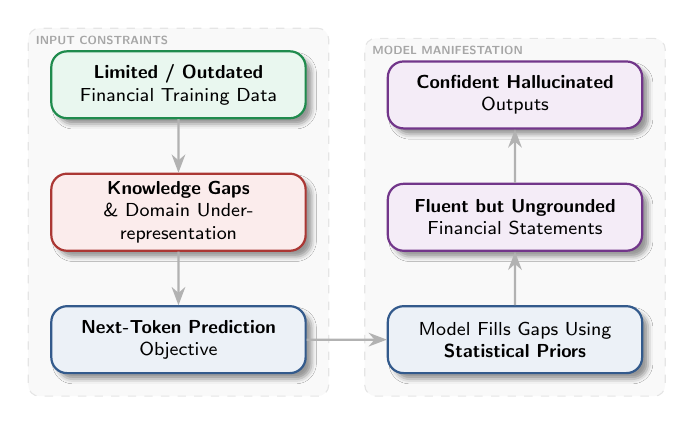
\begin{tikzpicture}[
    % GLOBAL SCALE: Adjusts the entire image size
    transform shape, scale=0.85, 
    node distance=0.8cm and 1.2cm, % Vertical and Horizontal spacing
    % --- Compact Node Styles ---
    process/.style={
        rectangle, 
        rounded corners=2mm, 
        minimum width=3.8cm,      % Reduced width
        minimum height=1.0cm,     % Reduced height
        text centered, 
        text width=3.5cm,         % Text wrapping width
        font=\sffamily\footnotesize, % Smaller font
        draw=gray!40,
        thick,
        blur shadow={shadow blur steps=3}
    },
    inputStage/.style={process, fill=dataGreen!10, draw=dataGreen!80!black},
    gapStage/.style={process, fill=alertRed!10, draw=alertRed!80!black},
    mechStage/.style={process, fill=researchBlue!10, draw=researchBlue!80!black},
    resultStage/.style={process, fill=outcomePurple!10, draw=outcomePurple!80!black},
    arrow/.style={-{Stealth}, thick, draw=gray!60, rounded corners},
    groupLabel/.style={font=\bfseries\sffamily\tiny, color=gray!70, anchor=north west}
]

    % --- LEFT COLUMN (The Problem) ---
    % 1. Input (Top Left)
    \node (step1) [inputStage] {
        \textbf{Limited / Outdated} \\ 
        Financial Training Data
    };

    % 2. Gaps (Below 1)
    \node (step2) [gapStage, below=of step1] {
        \textbf{Knowledge Gaps} \\ 
        \& Domain Under-representation
    };

    % 3. Objective (Below 2)
    \node (step3) [mechStage, below=of step2] {
        \textbf{Next-Token Prediction} \\ 
        Objective
    };

    % --- RIGHT COLUMN (The Result) ---
    % 4. Priors (Right of 3 - Bottom Right)
    \node (step4) [mechStage, right=of step3] {
        Model Fills Gaps Using \\ 
        \textbf{Statistical Priors}
    };

    % 5. Fluent (Above 4)
    \node (step5) [resultStage, above=of step4] {
        \textbf{Fluent but Ungrounded} \\ 
        Financial Statements
    };

    % 6. Output (Above 5 - Top Right)
    \node (step6) [resultStage, above=of step5] {
        \textbf{Confident Hallucinated} \\ 
        Outputs
    };

    % --- Arrows (The U-Shape Flow) ---
    \draw [arrow] (step1) -- (step2);
    \draw [arrow] (step2) -- (step3);
    \draw [arrow] (step3) -- (step4); % The bridge across
    \draw [arrow] (step4) -- (step5); % Moving up
    \draw [arrow] (step5) -- (step6); % Moving up

    % --- Compact Background Grouping ---
    \begin{scope}[on background layer]
        % Left Group
        \node [fit=(step1)(step3), fill=gray!5, draw=gray!20, rounded corners, dashed, inner sep=8pt] (groupL) {};
        \node [groupLabel] at (groupL.north west) {INPUT CONSTRAINTS};
        
        % Right Group
        \node [fit=(step4)(step6), fill=gray!5, draw=gray!20, rounded corners, dashed, inner sep=8pt] (groupR) {};
        \node [groupLabel] at (groupR.north west) {MODEL MANIFESTATION};
    \end{scope}

\end{tikzpicture}
\end{document}